\documentclass{ctexart}
\usepackage{graphicx} 
\usepackage{listings}
\usepackage{enumerate}
\usepackage{inputenc}
\usepackage{float}
\usepackage[namelimits]{amsmath} %数学公式
\usepackage{amssymb}             %数学公式
\usepackage{amsfonts}            %数学字体
\usepackage{mathrsfs}            %数学花体
\usepackage{authblk}
\usepackage[a4paper,scale=0.9,hcentering,bindingoffset=8mm]{geometry}

\begin{titlepage}
	\title{MapReduce大数据实验-金庸的江湖} 
	\author{
		吴刚,吴德亚,吴晗,温宗儒
	} 
	\date{\today}
\end{titlepage}
\begin{document}
	\maketitle
	\renewcommand{\contentsname}{目录} %将content转为目录
	\tableofcontents
	%实验要求
	\section{实验要求及目标}
	通过对“金庸的江湖——金庸武侠小说中的人物关系的挖掘”,来学习与掌握MapReduce程序设计。通过本课程设计的学习,可以体会如何使用MapReduce完成一个综合性的数据挖掘任务,包括全流程的数据预处理、数据分析、数据后处理等。\par
	本次实验的具体流程如下:\par
	(1)数据预处理:利用分词技术将文章中人物名字保留下来,其余去掉。\par
	(2)特征抽取:人物同现统计。\par
	(3)特征处理:人物关系图构建与特征归一化。\par
	(4)数据分析:基于人物关系图进行PageRank计算或者标签传播。\par
	(5)数据可视化及分析。\par
	
	% 任务分配
	\section{任务分配}
	\par 161220137\quad 吴刚\quad :任务三,任务五,数据可视化及相应报告书写
	\par 161220135\quad 吴德亚\quad :任务四,相应报告书写及latex报告转换
	\par 161220138 \quad 吴晗\quad	:任务一及相应报告书写
	\par 161220133 \quad 温宗儒\quad :任务二及相应报告书写
	
	% 实验环境		
	\section{实验环境}
	(1)Ubuntu1604 \par
	(2)Intellij IDEA 2018 \par
	(3)JDK 1.7\_79 \par
	(4)hadoop 2.7.1\par
	%实验过程		
	\section{实验过程}
	\subsection{一\quad 数据预处理}
	\par 本任务的主要工作是从原始的金庸小说文本中,抽取出不人物互动相关的数据,而屏蔽掉不人物关系无关的文本内容,为后面的基于人物共现的分析做准备。
	\subsubsection{任务简述}
	\par 数据输入:1.全本的金庸武侠小说文集(未分词);2. 金庸武侠小说人名列表。 
	\par 数据输出:分词后,仅保留人名的金庸武侠小说全集。
	\par 此处按照要求,对每一个小说文本生成一个仅包含人名的文件(格式:bookname-r-0000)
	
	\subsubsection{任务原理}
	\begin{enumerate}[I]
		\item \textbf{中文分词及Map的处理}
		\par 利用ansjseg 工具实现中文分词,ansjseg 支持对中文文本迚行分词,并且可以添加用户自定义的词典,这样就可以把出现在金庸小说里的人物的名字找出来。
	    而且在这里我们使用 \textbf{DistributeCache} 存储人名列表。
	\begin{lstlisting}[language=java, numbers=left, numberstyle=\tiny, frame=shadowbox, basicstyle=\ttfamily, escapeinside=``] 
`输入:文本段落 value`
`输出:`(bookname, names in this value-paragraph of this book)		
@Override
Method setup(context):
	file <- getCacheFiles()
	while (line <- readFile(file)) not null:
		wuxiaNameList.add(line)
		DicLibrary.insert(line)
		// Self-defined dictionary

Method map(key, value, context)
	filename <- context.getFileName()
// get the filename which paragraph belongs to
	termsList <- ToAnalysis.parse(value)
// the names List of paragraph
	for term in termsList:
		if term.isNR and wuxiaNameList.contains(term):
			result.add(term, '\t')
	if result.length > 0
		context.write(filename, result)
	\end{lstlisting}
	\par ParMapper类在setup函数中获取\textbf{Distributed Cache}中的人名列表,并在map函数中对段落中的人名分割,只有当人名出现在列表中时,才加入结果。
	\par 将人名列表传入Mapper/Reducer 有三种处理方法:
	\par 1. 转化成字符串通过Configuration()传递,适用于少量数据 
	\par 2. 通过Distributed Cache机制,\textbf{适合本实验}的namelist.txt传递 
	\par 3. 存储到HDFS,在Map/Reduce中读取HDFS,适用于大量数据。
	\item \textbf{多文件输出及Reduce处理}
	\begin{lstlisting}[language=java, numbers=left, numberstyle=\tiny, frame=shadowbox, basicstyle=\ttfamily, escapeinside=``] 
`输入:` filename, names in paragraph
`输出:` each book has a outputfile which contains names
Method reduce(key, <Text>values, context)
	for val in values:
		multiOutputs.write(val, "", key)
	\end{lstlisting}	
	\par 由于需要给每一本小说生成一个包含该小说所有人物的文件,故需要使用 \textbf{MultiOutput} 类。本次实验由于会生成多个文件,故使用第一个函数(后续的两个函数需要在main函数中制定 \textbf{addNamedOutput})
	\begin{lstlisting}[language=java, numbers=left, numberstyle=\tiny, frame=shadowbox, basicstyle=\ttfamily, escapeinside=``] 
void write(KEYOUT key, VALUEOUT value, String baseOutputPath)
	
<K, V> void write(String namedOutput, K key, V value)
	
<K, V> void write(String namedOutput, K key, V value, String baseOutputPath)
	\end{lstlisting}
	\par 需要注意的是:\textbf{在setup函数中进行初始化,在cleanup函数中关闭输出。}
	
	\end{enumerate}
	\subsubsection{运行结果}

	\begin{figure}[H]
		\centering
		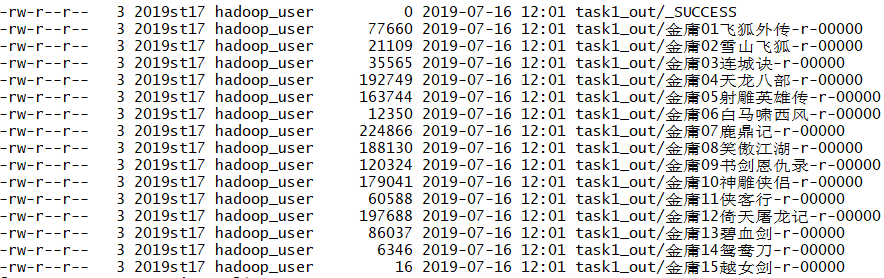
\includegraphics[width=0.8\linewidth]{pic/task1/filestyle}
		\caption{多文件输出列表}
	\end{figure}
	\begin{figure}[H]
	\centering
	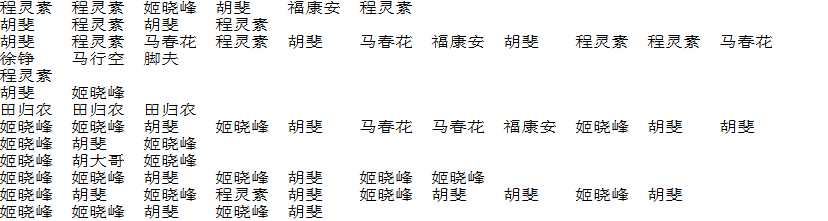
\includegraphics[width=0.8\linewidth]{pic/task1/filecontent}
	\caption{文件内容}
	\end{figure}
	\begin{figure}[H]
		\centering
		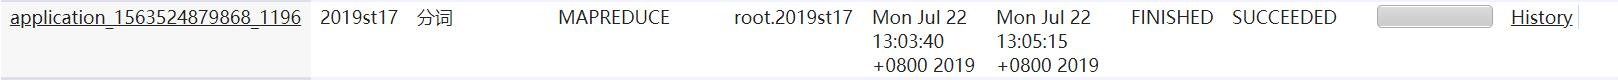
\includegraphics[width=0.8\linewidth]{pic/webui/task1}
		\caption{集群运行结果}
	\end{figure}
	\begin{figure}[H]
		\centering
		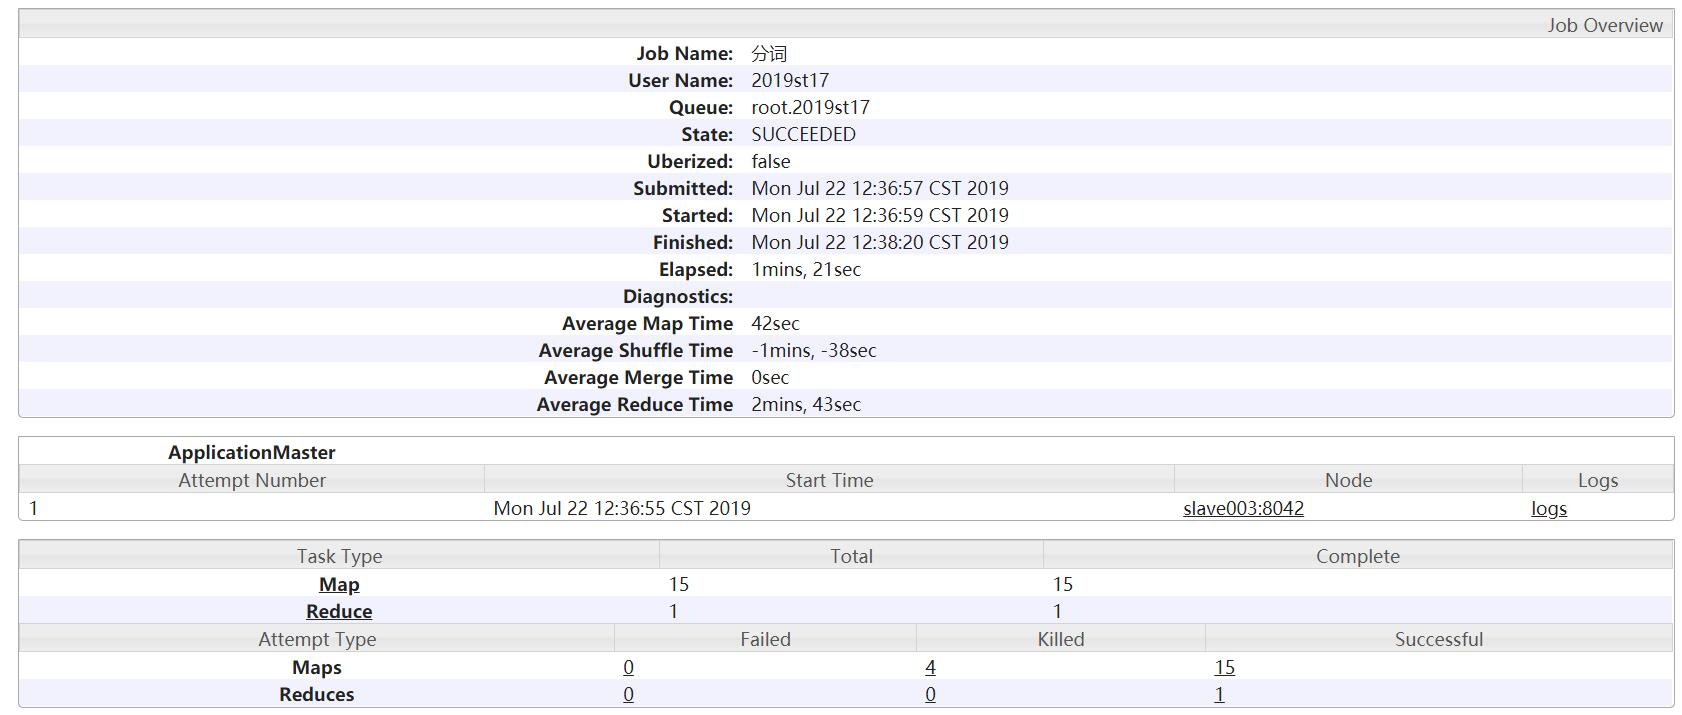
\includegraphics[width=0.8\linewidth]{pic/webui/task1_job}
		\caption{集群History}
	\end{figure}
	
	

	\subsection{二\quad 特征抽取:人物同现统计}
	\par 本任务的重要完成基于单词同现算法的人物同现统计。在人物同现分析中,如果两个人在原文的同一段落中出现,则认为两个人发生了一次同现关系。我们需要对人物之间的同现关系次数迚行统计,同现关系次数越多,则说明两人的关系越密切。
	\subsubsection{任务简述}
	\par 任务2分为图\ref{fig:map},图\ref{fig:reduce},首先读取任务1的输出,去除重复名字后,遍历所有组合,将其数字设为1;第二步,将所有键值相同的组合累加,输出每个键值出现的总次数。

	\subsubsection{任务原理}
	\par 使用\textbf{HashSet}去除重复人名,再进行人名的两两组合
	\begin{lstlisting}[language=java, numbers=left, numberstyle=\tiny, frame=shadowbox, basicstyle=\ttfamily, escapeinside=``] 
`输入:分词后仅保留人名的金庸武侠小说全集(每行表示一个段落)`
`输出:key: <name1, name2> value: 1`
Method Map(value):
	array[] <- value.split('\t')
	for all t in array[]:
		for all u in array[]:
			emit(<t, v>, one) 

`输入:key: <name1, name2> value: 1`
`输出:key: <name1, name2> value:同现次数`
Function Reduce(key, values[])
	for val in values:
		sum += val
	emit(key, sum)
	\end{lstlisting}
	
		\begin{figure}[H]
		\centering
		\begin{minipage}[t]{0.3\textwidth}
			\centering
			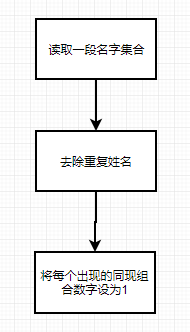
\includegraphics[width=0.9\linewidth]{pic/task2/map}
			\caption{Map}
			\label{fig:map}
		\end{minipage}
		\begin{minipage}[t]{0.6\textwidth}
			\centering
			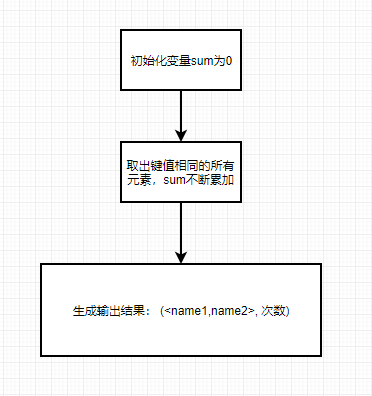
\includegraphics[width=0.9\linewidth]{pic/task2/reduce}
			\caption{Reduce}
			\label{fig:reduce}
		\end{minipage}
	\end{figure}

	\subsubsection{运行结果}
	\begin{figure}[H]
		\centering
		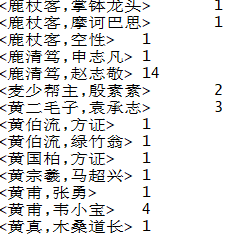
\includegraphics[width=0.3\linewidth]{pic/task2/result}
		\caption{输出文件格式}
	\end{figure}
	\begin{figure}[H]
	\centering
	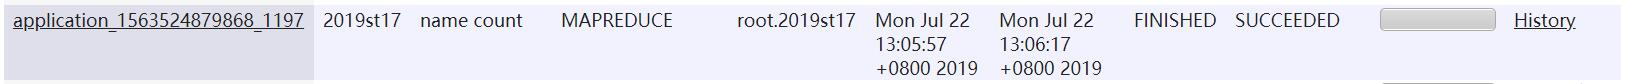
\includegraphics[width=0.8\linewidth]{pic/webui/task2}
	\caption{集群运行结果}
	\end{figure}
	\begin{figure}[H]
	\centering
	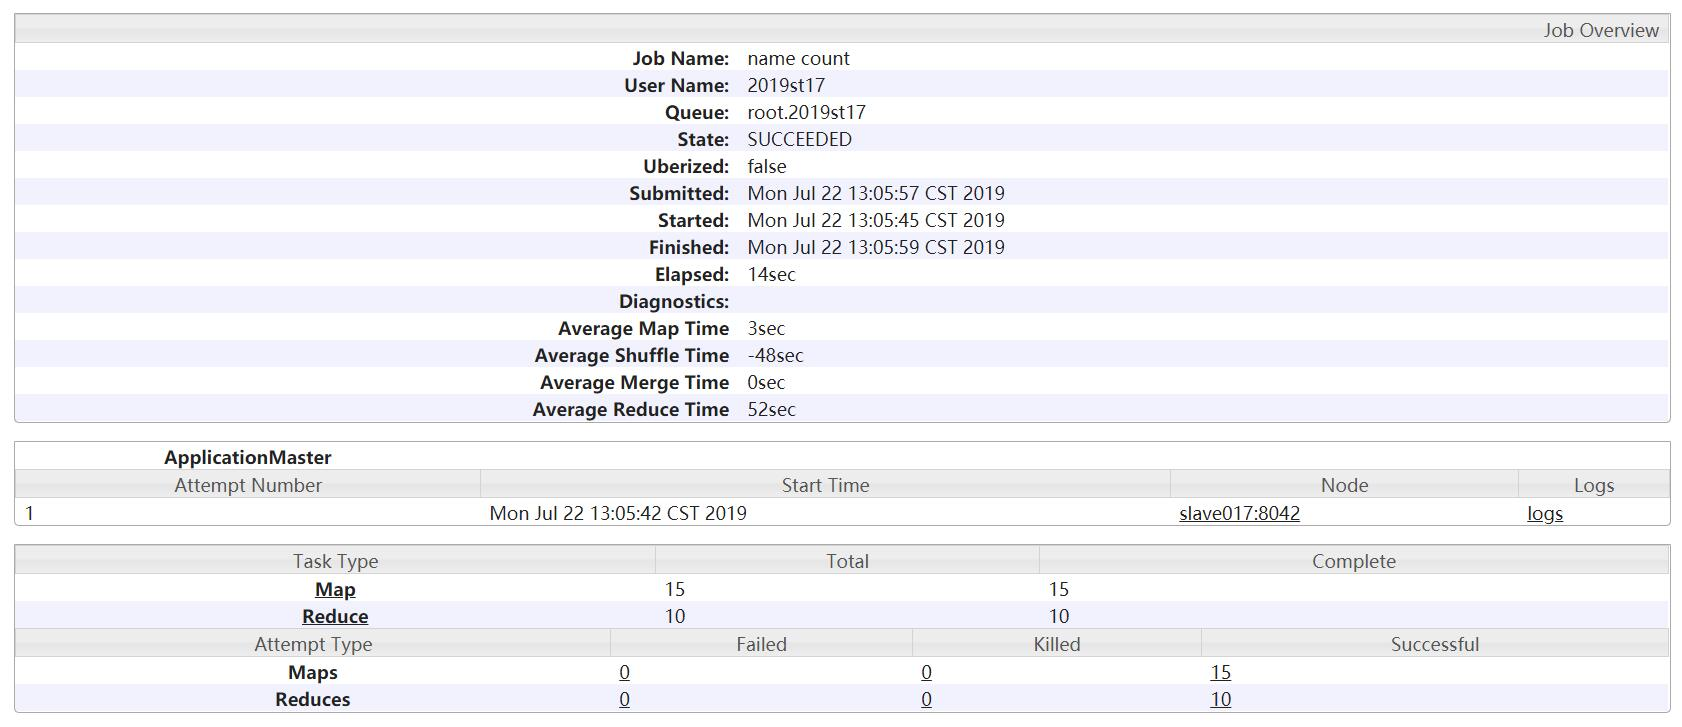
\includegraphics[width=0.8\linewidth]{pic/webui/task2_job}
	\caption{集群History}
	\end{figure}
	
	\subsection{三\quad 特征处理:人物关系图构建不特征归一化}
	\subsubsection{任务简述}
	当获取了人物之间的共现关系之后,我们就可以根据共现关系,生成人物之间的关系图了。人物关系图使用邻接表的形式表示,方便后面的PageRank计算。在人物关系图中,人物是顶点,人物之间的互劢关系是边。人物之间的互劢关系靠人物之间的共现关系确定。如果两个人之间具有共现关系,则两个人之间就具有一条边。两人之间的共现次数体现出两人关系的密切程度,反映到共现关系图上就是边的权重。边的权重越高则体现了两个人的关系越密切。\par
	为了使后面的方便分析,还需要对共现次数迚行归一化处理:将共现次数转换为共现概率。 \\ 
	\par 数据输入:任务二的输出
	\par	数据输出:归一化后的人物关系图
	\subsubsection{任务原理}
	\begin{lstlisting}[language=java, numbers=left, numberstyle=\tiny, frame=shadowbox, basicstyle=\ttfamily, escapeinside=``] 
Mapper
`输入:key:<name1,name2> value:同现次数`
`输出:key:name1 value:<name2,同现次数>`
Function map(Text key, Text value):
	name1, name2 <- key
	Emit(name1, <name2,value>)

Reduce
`输入:key:name  value:列表,里面每个元素为<name2, n>`
`输出:key:name  value: 字符串 ”name2,n2|name3,n3|…”`
Function reduce(Text key, list<Text> values):
	postList <- new 一个字符串列表
	sum <- 0
	for all value in values: 
		postList.append(value)
		name2, n <- value
		sum += n
	realValue <- “”
	for all value in postList:
		name2, n <- value
		realValue += (name2 + “,” + n / sum + “|”)
	realValue[last] <- “]”
	realValue <- “[” + realValue
	Emit(name, realValue)


	\end{lstlisting}
	\subsubsection{运行结果}
	\begin{figure}[H]
		\centering
		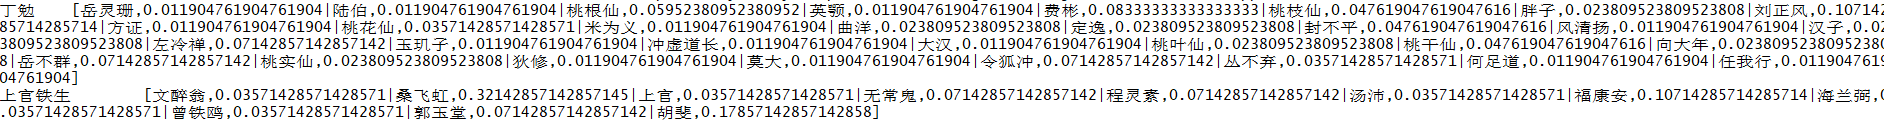
\includegraphics[width=0.8\linewidth,height=0.1\linewidth]{pic/task3/result}
		\caption{输出文件格式}
	\end{figure}
	\begin{figure}[H]
	\centering
	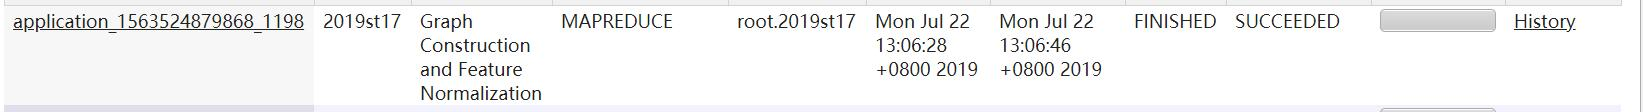
\includegraphics[width=0.8\linewidth]{pic/webui/task3}
	\caption{集群运行结果}
	\end{figure}
	\begin{figure}[H]
	\centering
	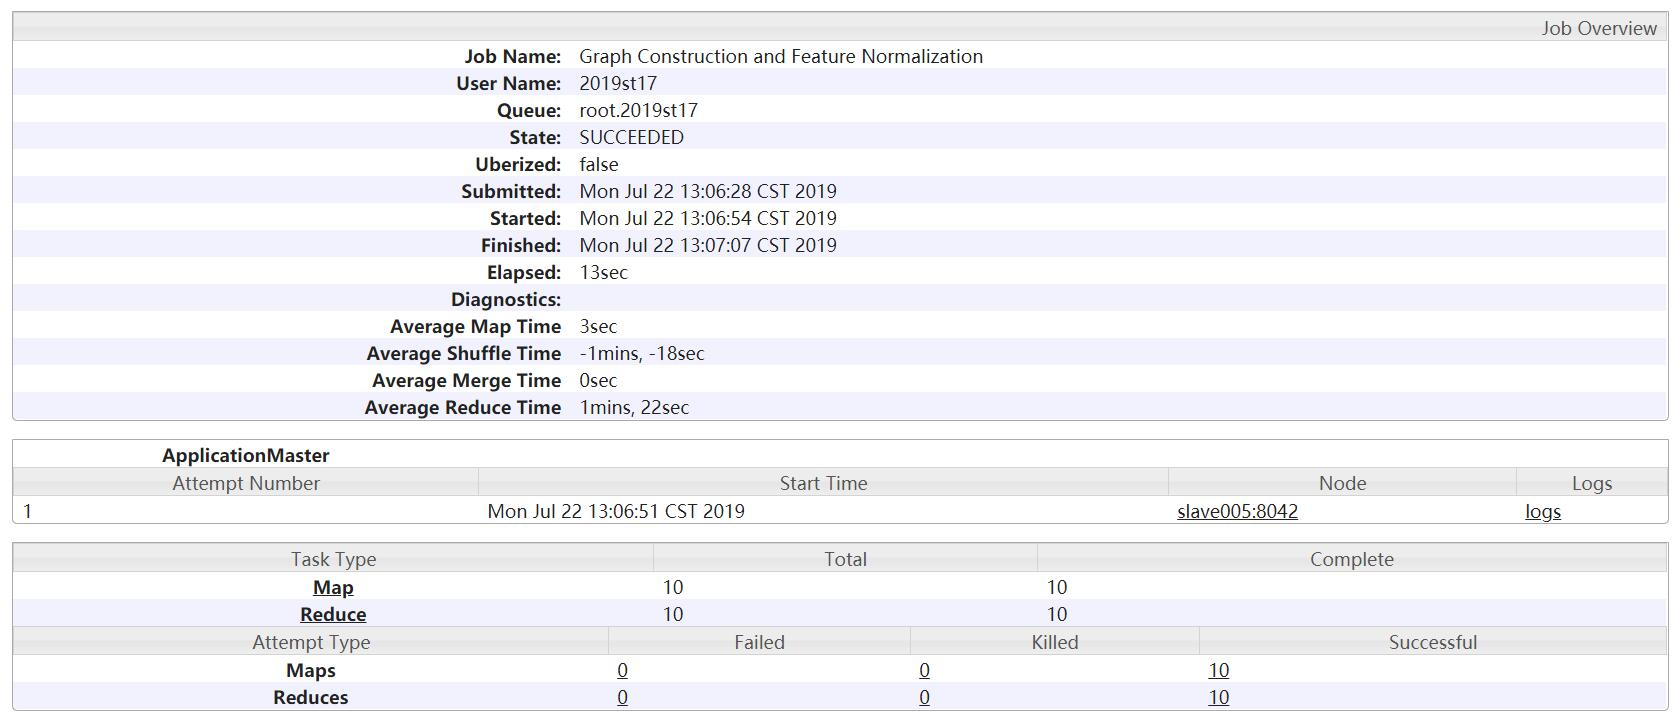
\includegraphics[width=0.8\linewidth]{pic/webui/task3_job}
	\caption{集群History}
	\end{figure}

	% 任务4
	\subsection{四\quad 数据分析:基于人物关系图的PageRank计算}
	\subsubsection{任务简介}
	\par 在这一部分,需要实现的功能是:对任务关系图进行一个数据分析,通过PageRank,
	我们就可以定量地分析金庸武侠江湖中的“主角”们是哪些。PageRank任务总共分为三个部分,首先将获取的数据格式化为能够处理的格式,其次进行迭代运算,最后将结果进行整理。
	\par 共分为4个类,\textbf{CorrectFormat.class, PageRanking.class, SortPageRank.class, PageRankDriver.class}
	\subsubsection{实验原理}
	\begin{enumerate}[I]
		\item \textbf{Driver主函数}
		\par 函数调用顺序如图\ref{fig:drivercall}:前一轮的输出为后一轮的输入,PageRanking会迭代执行,直到满足条件:(人物排名不再改变或迭代固定次数,在这里我们使用固定次数 \textbf{TIMES})
		\begin{figure}[H]
			\centering
			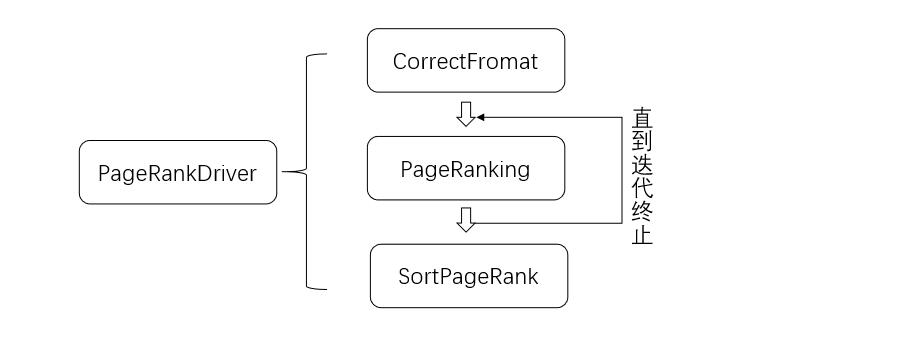
\includegraphics[width=0.7\linewidth]{pic/task4/driverCall}
			\caption{主函数框架}
			\label{fig:drivercall}
		\end{figure}
	
		\item  \textbf{调整数据格式} 
		\par 任务3的输出格式如图\ref{fig:task4cf};
			经过格式修改后得到的格式如图\ref{fig:task3output}(其中PR\_INIT即为每个人物PR的初始值)。
		\begin{figure}[H]
			\centering
			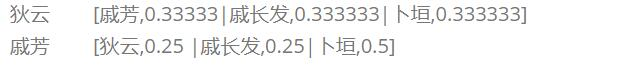
\includegraphics[width=0.7\linewidth]{pic/task4/task3output}
			\caption{格式修改前}
			\label{fig:task4cf}
		\end{figure}
		\begin{figure}[H]
			\centering
			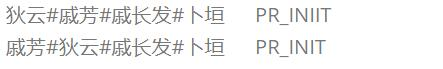
\includegraphics[width=0.7\linewidth]{pic/task4/task4CF}
			\caption{格式修改后}
			\label{fig:task3output}
		\end{figure}
		\par \textbf{Map} 函数的处理 (key, value的选取)
		\begin{lstlisting}[language=java, numbers=left, numberstyle=\tiny, frame=shadowbox, basicstyle=\ttfamily, escapeinside=``] 
`输入:` name [name,heavy|name,heavy]
`输出:` (name#name#name PR\_INIT)
Method Map(Text value, Context context):
	leaderName <- value.toString.split(`' '`)[0]
	followItems <- value.toString.split(`' '`)[1] 
	// get list (name, heavy)
	String[] followName <- followItems.split('|' or '[') 
	StringBuilder result <- new StringBuilder();
	for items in followName[]:
		name <- items.split(',')[0]
		if name.length > 0:
			result.append('#' + name)
	context.write(Text(result), PR_INIT)	
	// name_link list and PR value
		
		\end{lstlisting}
		\par \textbf{Reduce} 函数按照接收的key, value写入文件即可.
		
		
		
		\item \textbf{迭代PageRank}
		\par 由于需要进行迭代,故每次写入的文件格式都与\textbf{4.2}的输出格式相同。
		\par \textbf{Map} 函数的处理: 
		\begin{lstlisting}[language=java, numbers=left, numberstyle=\tiny, frame=shadowbox, basicstyle=\ttfamily, escapeinside=``]

`输入:` name#name#name valuePR
`输出:` (name+valuePR one) OR	(name#name#name one)
Method Map(Text value, Context context):	
	names <- value.toString.split('\t')[0]
	// get name_link_list
	pr <- value.toString.split('\t')[1]
	// get pr value
	items[] <- names.split('#')
	leaderPR <- pr.value / len(items.length-1)
	for i = 1 to items.length:
		temp <- items[i] + leaderPR
		context.write(Text(temp), 1)
	context.write(Text(names), 1)
		\end{lstlisting}
	\par 在最后仍然需要给出人物的链接关系,以免丢失信息,便于下一次的迭代 
	
	\par \textbf{NewPartitioner}自定义Partition函数,将键值对分组到Reduce中。
		\begin{lstlisting}[language=java, numbers=left, numberstyle=\tiny, frame=shadowbox, basicstyle=\ttfamily, escapeinside=``]
		
`输入:` (name+valuePR one) OR	(name#name#name one)
`操作: 找出两者的第一个name,并作为参数调用父类的getPartition函数` 
`输出:` (name+valuePR one) OR	(name#name#name one)
@Override
Method int getPartition(key, value)
	if key.toString.contains('+'):
		term <- key.toString.split('+')[0]
	else
		term <- key.toString.split('#')[0]
	return super.Partition(term, value)	
			
		\end{lstlisting}
	\par 如果key中包含'+',则表明是 name+pr 的结构,否则即为 name\_link\_list 的结构;需要保证的是:后者的出发节点和前者的人物在同一个Reduce任务中 
		
		\par \textbf{Reduce} 函数的处理:	
		
		\begin{lstlisting}[language=java, numbers=left, numberstyle=\tiny, frame=shadowbox, basicstyle=\ttfamily, escapeinside=``]
`输入:` (name+valuePR one) OR	(name#name#name one)
`输出:` (name#name#name  valuePR)
Method Reduce(key, values, context)
	//get leaderName as NewPartition's term
	leaderName <- key.getLeaderName
	initialize cur <- leaderName
	// just do it once
	if not cur.equals(leaderName):
		cleanup(context)
	// call the cleanup to write info
	if key.toString.contains('+')
	// key format: name+pr
		for v in values[]:
			valuePR += (PR in key)
	// the same name+pr may accur several times
	else:
		linkList <- key.toString()
	// key format: name#name#name
		
@Override 
Method cleanup(context)
	valuePR <- (1-PR\_CHANGE)+PR\_CHANGE*valuePR
	context.write(linkList, valuePR)
	// emit format: name#name#name	valuePR
	valuePR <- 0
		\end{lstlisting}
	\par 重载cleanup函数,当发现接收到的key值中的leaderName发生变化时,表明:上一个leaderName的PR已经计算完成
	,需要将其保存,保存的格式为:name\_link\_list '\t' valuePR 
		
		\item \textbf{ 数据排序}
		\par 1. 在Map函数中以每个人物的pr值作为key,人名为value发送出去,经过默认的partition函数发给Reduce任务(在这里,我们设置Reduce任务的个数为1)
		\par 2. 在 Reduce 函数中重写 DoubleWritable.Comparator 类的 comapre函数。
	

		\begin{lstlisting}[language=java, numbers=left, numberstyle=\tiny, frame=shadowbox, basicstyle=\ttfamily, escapeinside=``]
@Override
Method compare(byte[] b1, int s1, int l1, 
		 byte[] b2, int s2, int l2) 
    return -super.compare(b1, s1, l1, b2, s2, l2);
		\end{lstlisting}	
		\par 3. 最后,在Reduce函数中按照key, value的顺序写入文件即可。
	\end{enumerate}
	
	\subsubsection{运行结果}
	\begin{figure}[H]
		\centering
		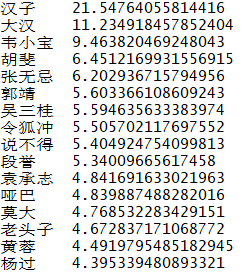
\includegraphics[width=0.3\linewidth]{pic/task4/Result}
		\caption{输出文件格式}
	\end{figure}
	\begin{figure}[H]
		\centering
		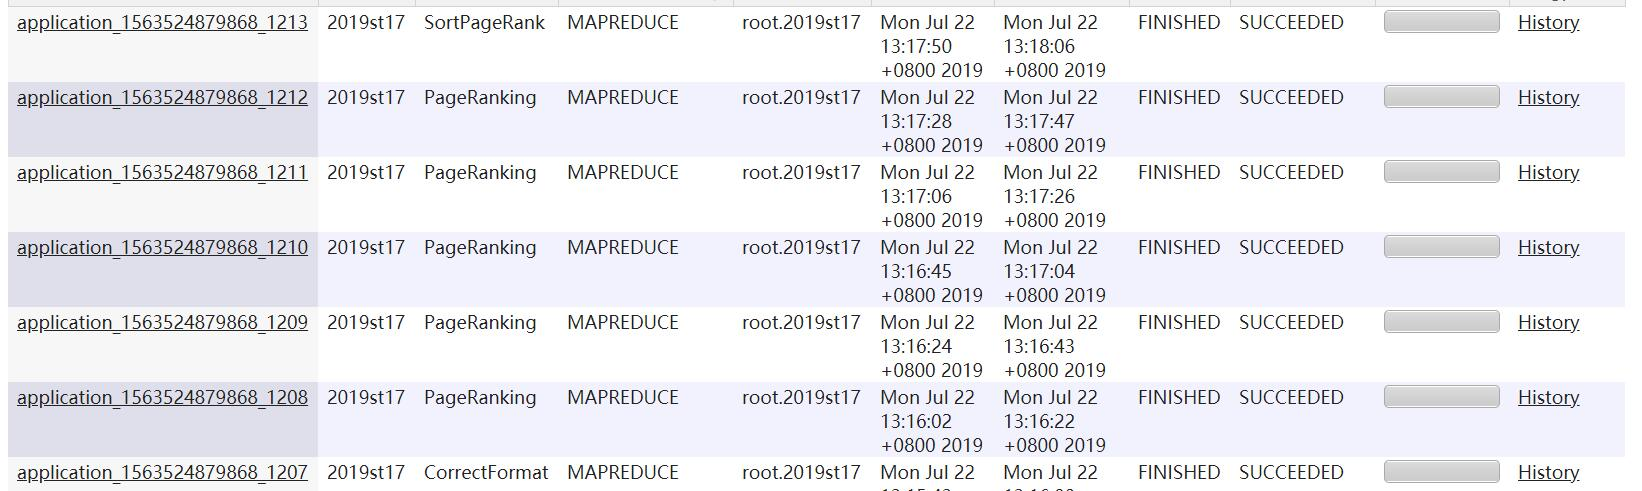
\includegraphics[width=0.8\linewidth]{pic/webui/task4}
		\caption{集群运行结果}
	\end{figure}
		\begin{figure}[H]
		\centering
		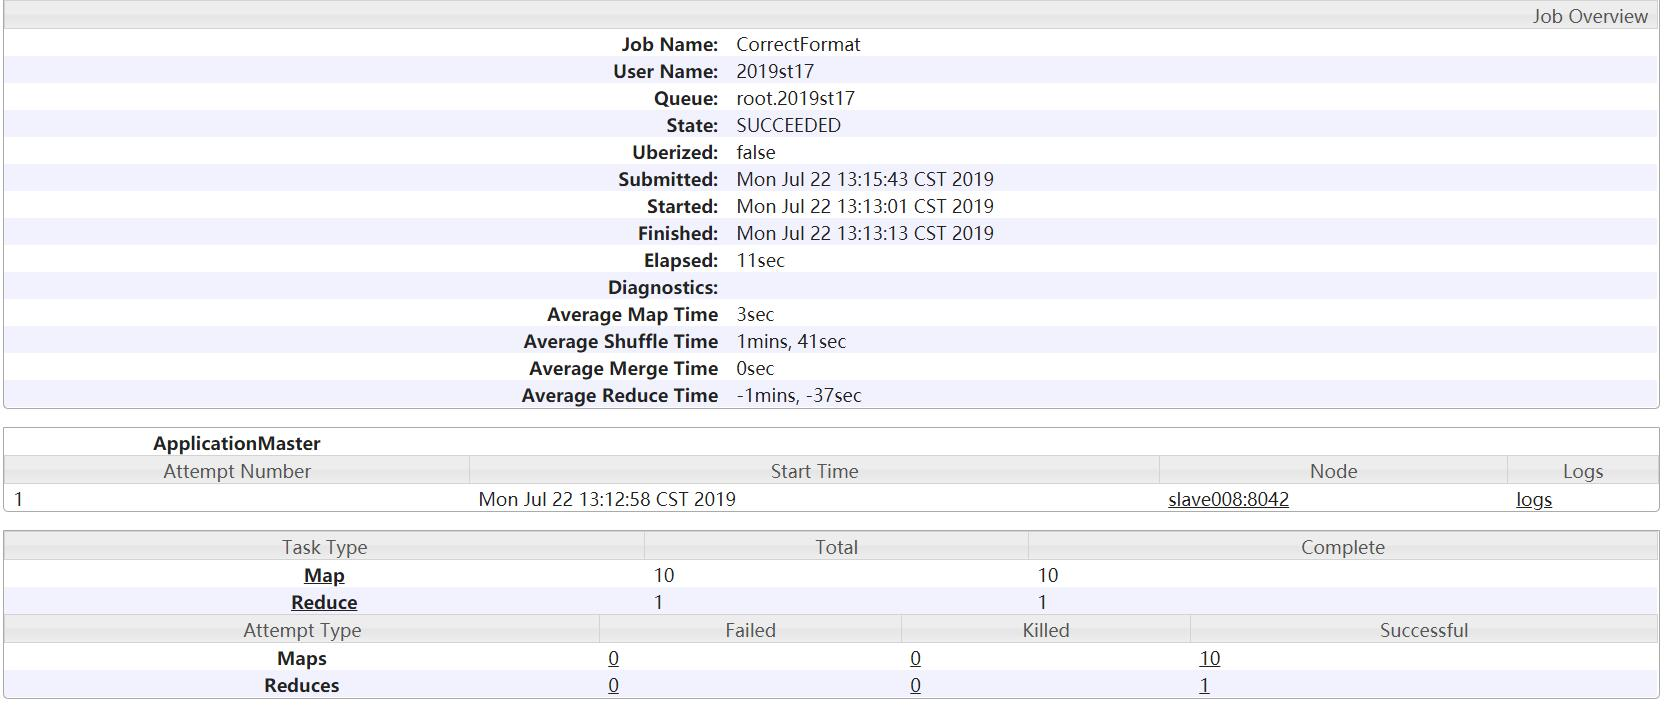
\includegraphics[width=0.8\linewidth]{pic/webui/task4_job1}
		\caption{集群 \textbf{CorrectFormat} History}
	\end{figure}
	\begin{figure}[H]
	\centering
	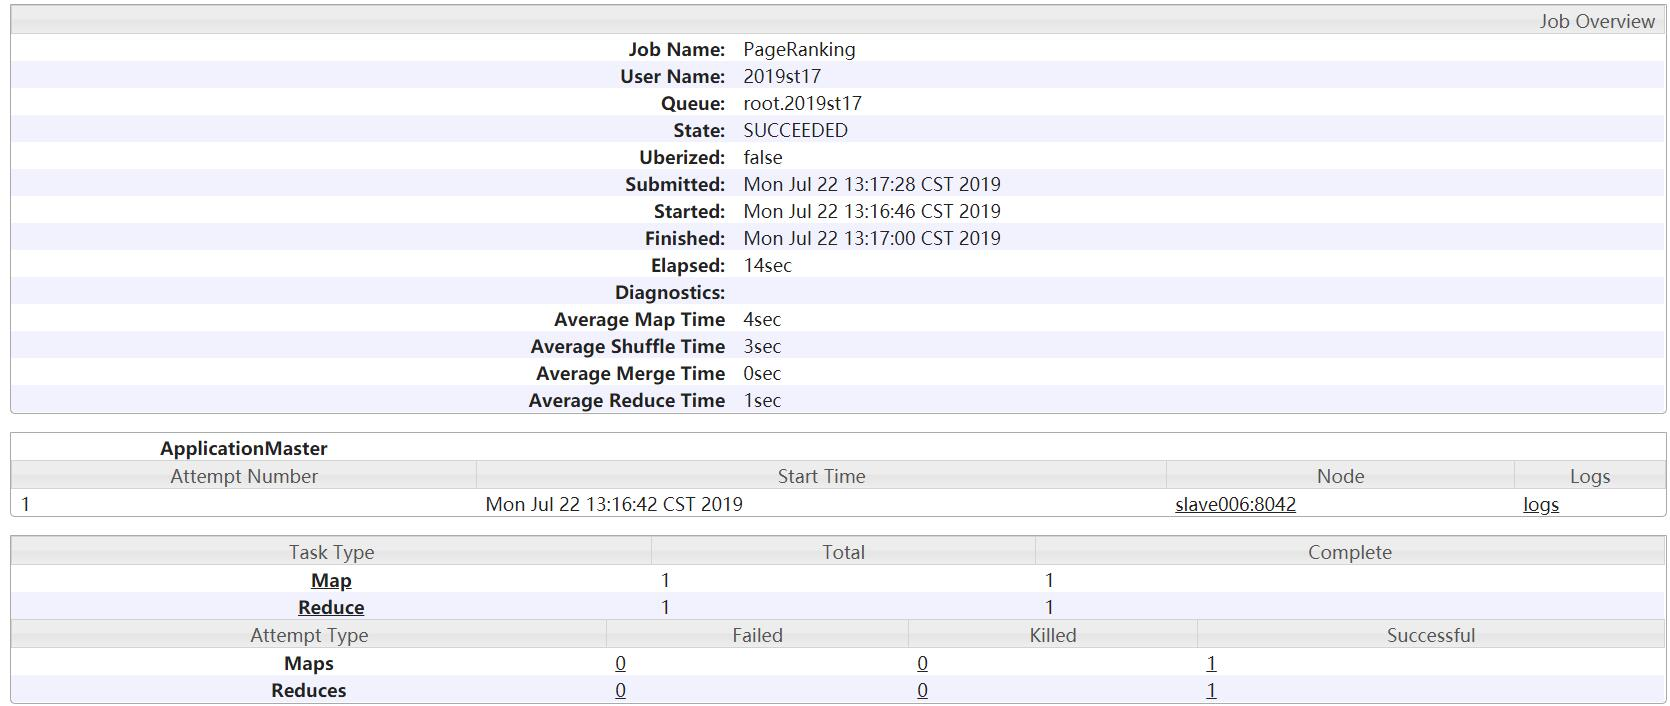
\includegraphics[width=0.8\linewidth]{pic/webui/task4_job2}
	\caption{集群\textbf{PageRank}History}
\end{figure}
	\begin{figure}[H]
	\centering
	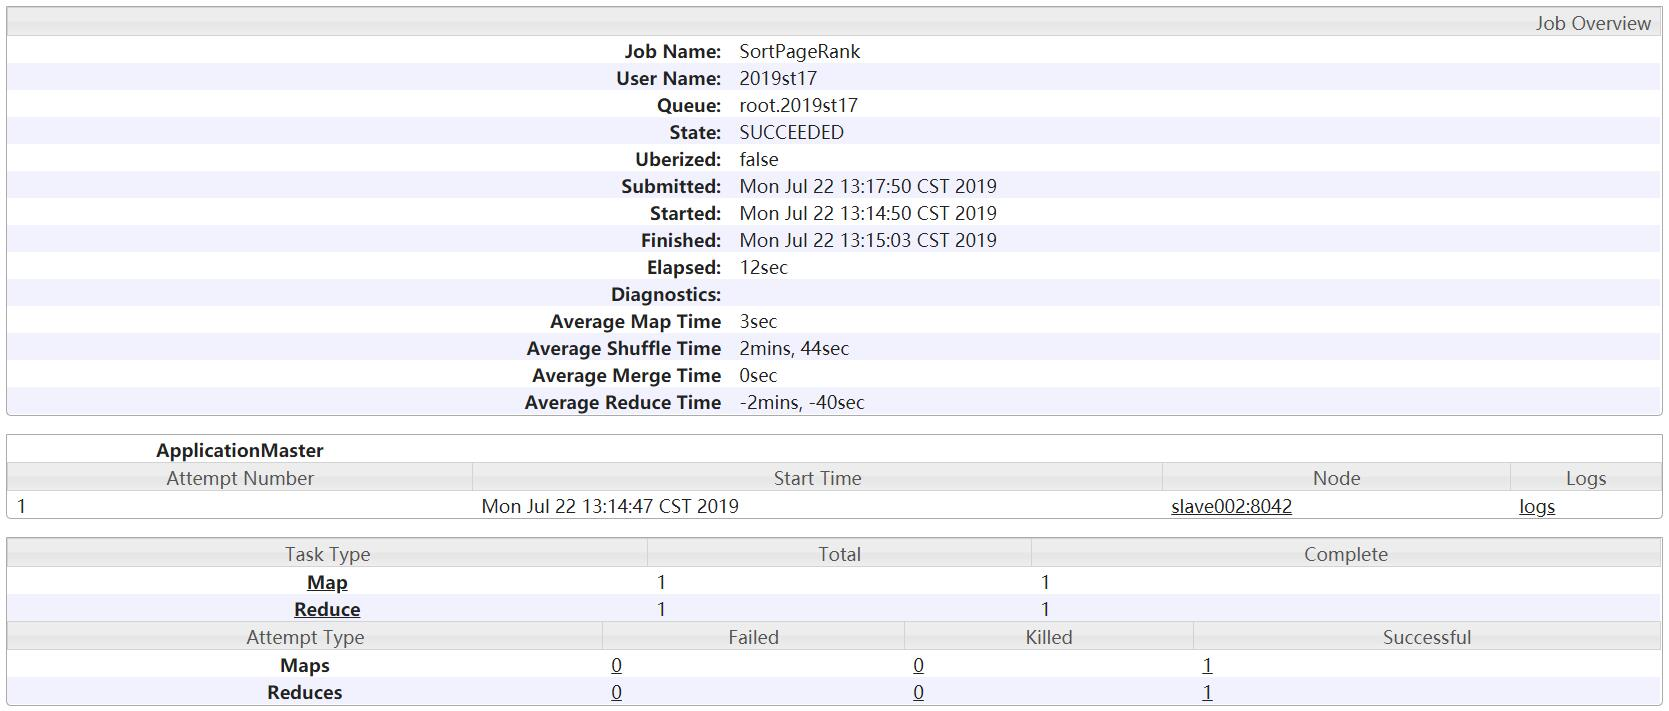
\includegraphics[width=0.8\linewidth]{pic/webui/task4_job3}
	\caption{集群\textbf{SortPageRank}History}
\end{figure}

	
	\subsection{五\quad 数据分析:人物关系图的标签传播}
	\subsubsection{任务简述}
	\par 标签传播(LabelPropagation)是一种半监督的图分析算法,他能为图上的顶点打标签,迚行图顶点的聚类分析,从而在一张类似社交网络图中完成社区发现(Community Detection)。将金庸小说中的人物完成社区发现。
	\par 输入:任务3的输出,人物之间的连接关系
	\par 输出:人物及其标签
	\subsubsection{任务原理}
	\par 标签传播可以分成以下三步骤:
	\begin{enumerate}[I]
		\item \textbf{数据标准化}
		\par 这与任务三有点像:不同点在于:未归一化并且人物都会有一个标签。格式为:
		\par name, label Link
		\par 其中Link为其相邻点及其共现次数。name1,n1$\left|\text{}\right.$name2,n2$\left|\text{}\right.$name3,n3 以$\left|\text{}\right.$为分隔符
		\item \textbf{标签传播迭代}
		\begin{lstlisting}[language=java, numbers=left, numberstyle=\tiny, frame=shadowbox, basicstyle=\ttfamily, escapeinside=``]	
Mapper
`输入:key: name, label	
		value: name1,n1|name2,n2|name3,n3 `
`输出:key: name(i)	value:<name,label,ni> `
Function map(Text key, Text value):
	name, label <- key		
	for all one in value:
		name(i), n(i) <- one
		Emit(name(i), <name,label,n(i)>)
Reducer
`输入: key: name	value:以<name, label, ni>格式的列表`
`输出: key name, label	value: name1,n1|name2,n2|name3,n3`
Function reduce(Text text, list<Text> values):
	map <- new Map<String, int>()
	realValue = ""
	for all value in values:
		name,label,n <- value
		if(label in map.keys)
			map(label) = 0
		else
			map(label) += n
		realValue += (name+','+n+'|')
		label <- map `中的值的最大的key`
		Emit(<name,label>, realValue)

		\end{lstlisting}
		\item \textbf{统计标签}
		\par 当迭代收敛或者到达一定次数停止
		\par 将最后一次的结果转化成 label, name 的形式即可。
		
	\end{enumerate}
	\subsubsection{运行结果}
	\par 如图\ref{flagName},表示每个人物所属的人名,可以转换成便于查看的结果,如图\ref{nameFile}。
	\begin{figure}[H]
	\centering
	\begin{minipage}[t]{0.15\textwidth}
		\centering
		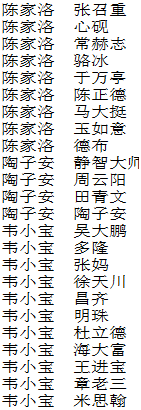
\includegraphics[width=0.9\linewidth]{pic/task5/LPA}
		\caption{标签\&人名}
		\label{flagName}
	\end{minipage}
	\begin{minipage}[t]{0.75\textwidth}
		\centering
		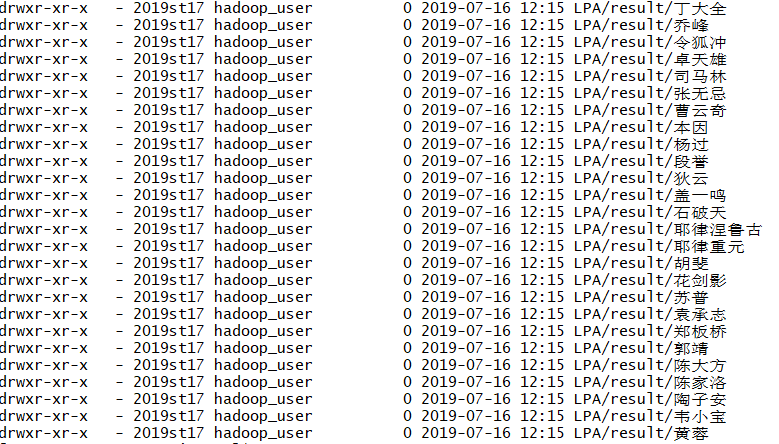
\includegraphics[width=0.9\linewidth]{pic/task5/Result}
		\caption{有相同标签的写入同一个文件}
		\label{nameFile}
	\end{minipage}
	\end{figure}
	\begin{figure}[H]
	\centering
	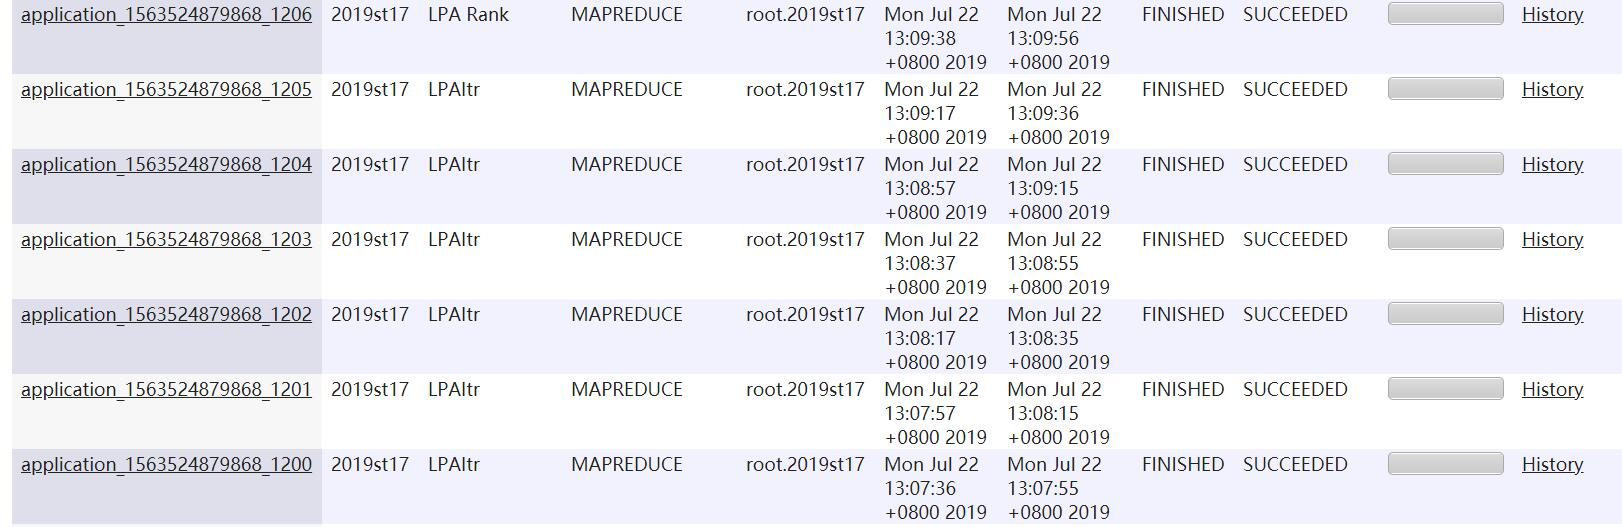
\includegraphics[width=0.8\linewidth]{pic/webui/task5}
	\caption{集群运行结果}
	\end{figure}
		\begin{figure}[H]
		\centering
		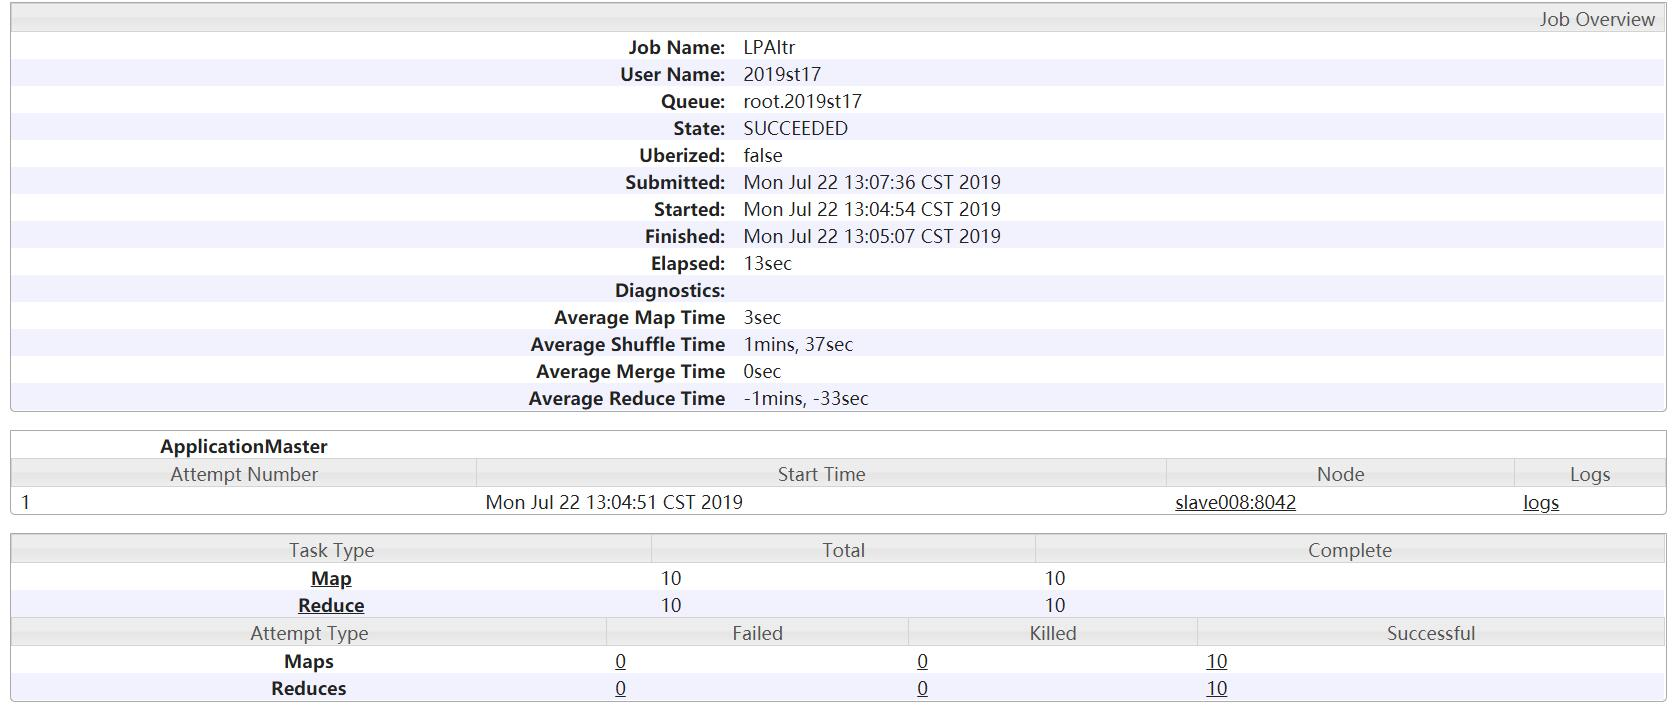
\includegraphics[width=0.8\linewidth]{pic/webui/task5_job1}
		\caption{集群\textbf{LPAltr}History}
	\end{figure}
	\begin{figure}[H]
	\centering
	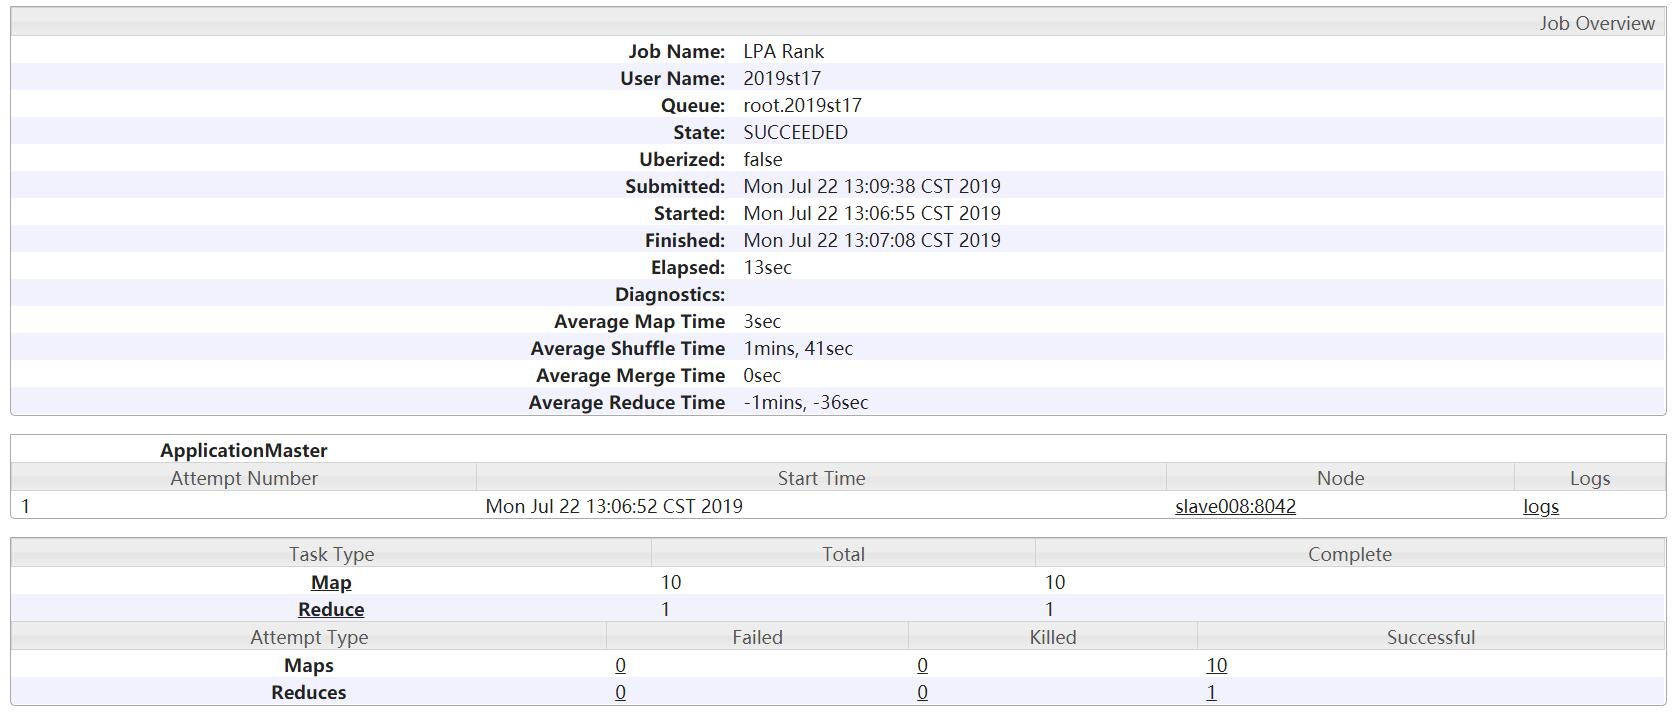
\includegraphics[width=0.8\linewidth]{pic/webui/task5_job2}
	\caption{集群\textbf{LPA Rank}History}
\end{figure}


	\subsubsection{数据可视化}
	\par 使用软件\textbf{Gephi},由给出的标签人物信息,自动生成图,更直观展示人物之间的关系。
	\par 通过如图\ref{getPointsEdges}指令获取人物顶点和边的关系,points.csv \& edges.csv,导入软件即可获取如图\ref{graphCircle}和图\ref{graphCircle2},局部放大图\ref{graphLocal}的效果
	\begin{figure}[H]
		\centering
		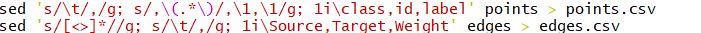
\includegraphics[width=0.8\linewidth]{pic/visible/Visible}
		\caption{获取边及顶点}
		\label{getPointsEdges}
	\end{figure}
	
	\begin{figure}[H]
		\centering
		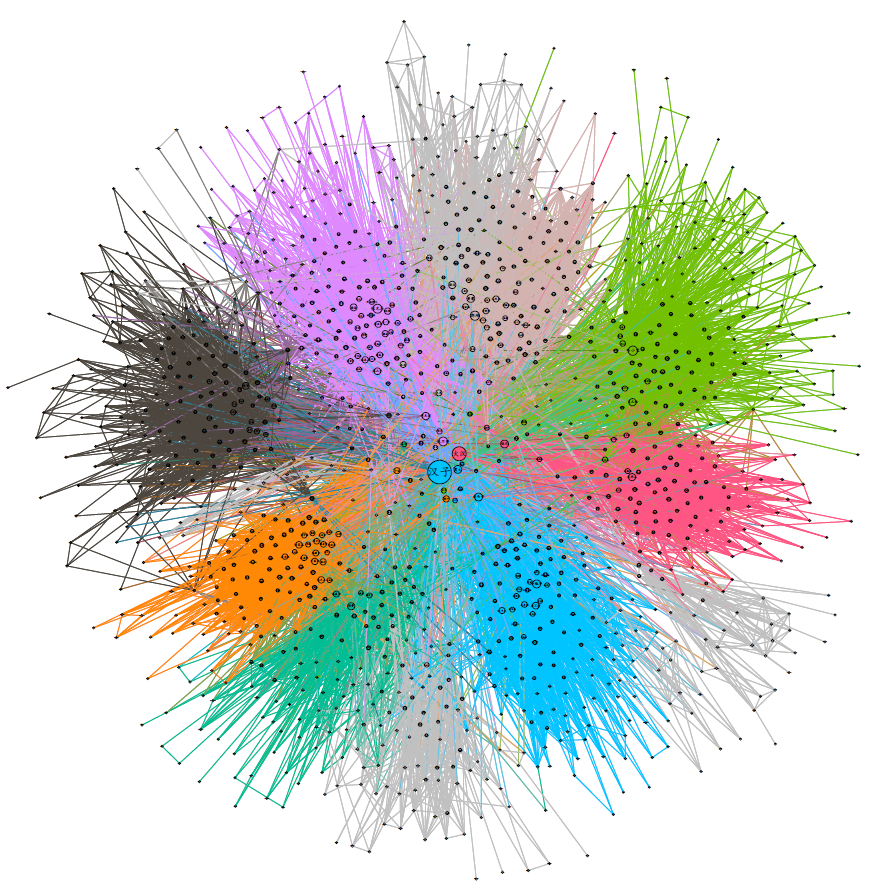
\includegraphics[width=0.65\linewidth]{pic/visible/Pic1}
		\caption{人物关系图}
		\label{graphCircle}
	\end{figure}
		\begin{figure}[H]
		\centering
		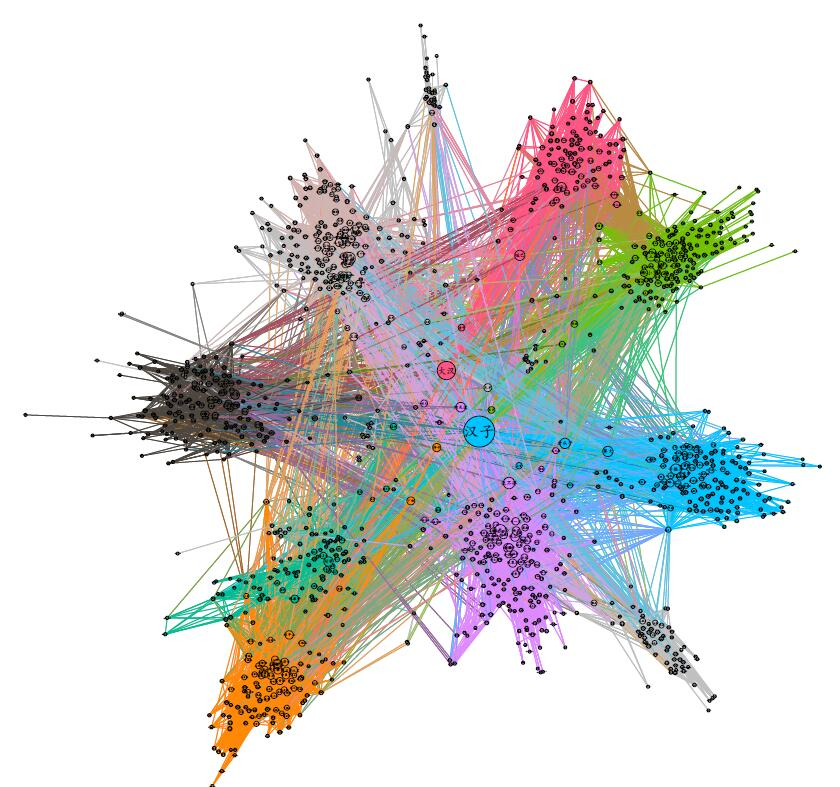
\includegraphics[width=0.65\linewidth]{pic/visible/another}
		\caption{人物关系图2}
		\label{graphCircle2}
	\end{figure}
	\begin{figure}[H]
		\centering
		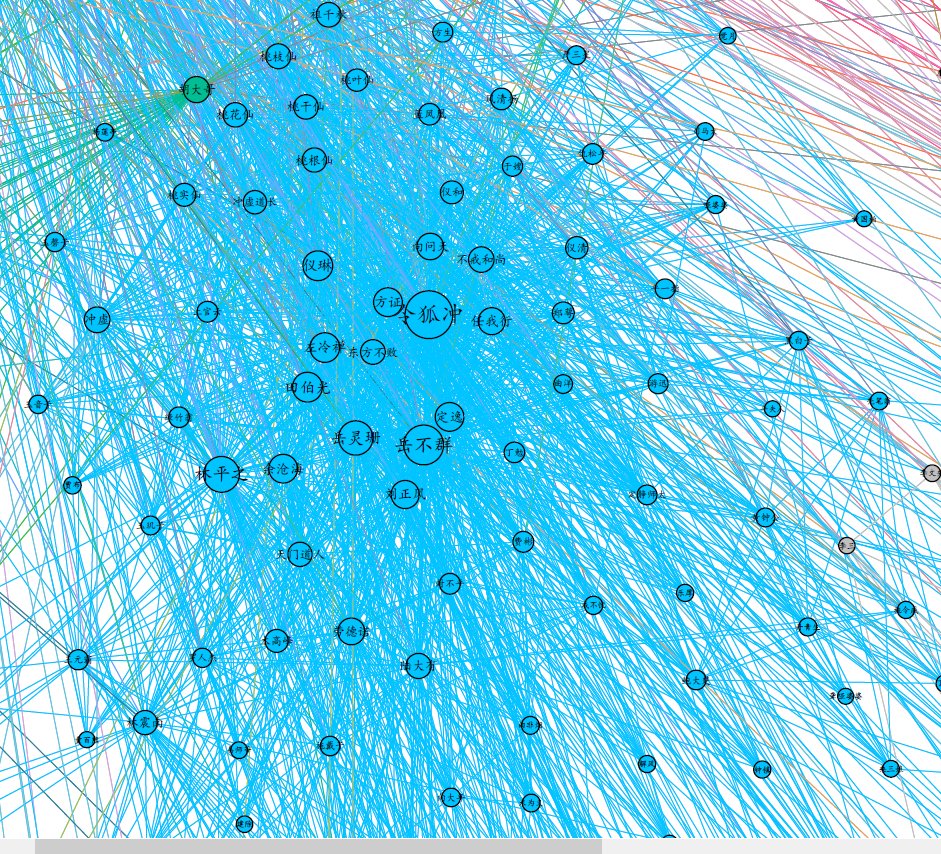
\includegraphics[width=0.7\linewidth]{pic/visible/Pic2}
		\caption{局部放大《笑傲江湖》}
		\label{graphLocal}
	\end{figure}
	
	
	
	
	
	\subsection{六\quad 分析结果整理}
	\subsubsection{任务简述}
	\par 任务4和任务5默认的输出内容是杂乱的,从中无法直接的得到分析结论,因此我们需要对上述分析的结果迚行整理、从而使人可以很容易地从分析结果中发现一些有趣的结论。
	\subsubsection{运行结果}
	\par 由于该任务涉及的\textbf{MultiOutput}多文件输出,定制\textbf{Partition}等原理在之前的任务中已经介绍过,故不再赘述
	\begin{enumerate}[I]
		\item 任务4输出,排序
		\begin{figure}[H]
			\centering
			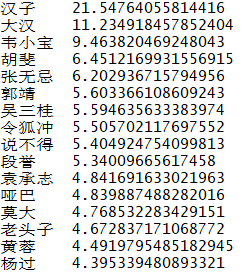
\includegraphics[width=0.3\linewidth]{pic/task6/PR}
			\caption{按照PR从大到小排序}
			\label{fig:pr}
		\end{figure}
		
		\item 任务6输出,将属于同一个标签的任务输出到一起,便于查看标签传播的结果
		\begin{figure}[H]
			\centering
			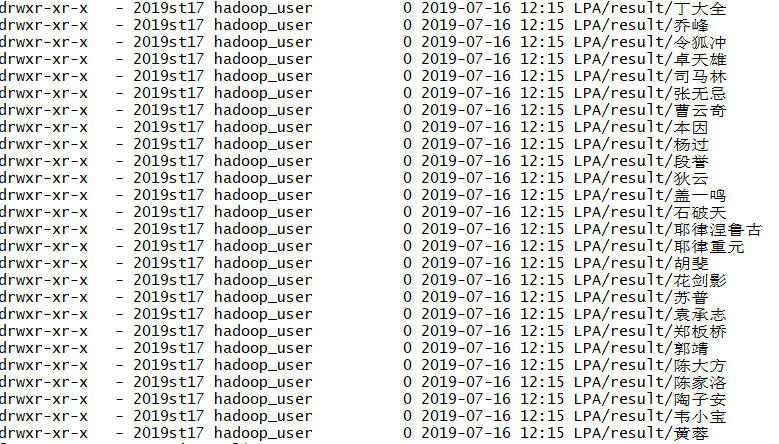
\includegraphics[width=0.8\linewidth]{pic/task6/LPA}
			\caption{属于同一个标签的在同一个文件中}
			\label{fig:lpa}
		\end{figure}
		
	\end{enumerate}
	
\section{实验心得体会}
\begin{enumerate}[I]
	\item 通过参与小组形式的实验,体验到成员合作的重要性,每个人都有分工,一起商讨问题的解决方案
	\item 善于从书本、网络上寻找Bug的解决方案,耐心调试
	\item 完成了一个使用mapreduce框架进行数据分析的流程,了解了基本步骤
\end{enumerate}

\section{致谢}
\par 感谢《大数据》这门课程的顾荣老师和助教们的答疑解惑,同时也感谢与我们组进行探讨交流的其他小组。
\par 最后谢谢小组各位成员的努力和付出,我们得以成功完成本门课程的大实验。
	
\end{document}